\section{Optimized Implementation for Dixon Resultant}\label{Section: Improvements}

While the theoretical complexity analysis highlights the advantages of Dixon resultant methods, bridging the gap to practical efficiency requires overcoming several significant hurdles. Currently, off-the-shelf computer algebra systems offer limited support: Dixon resultants are not natively implemented in advanced solvers like Magma~\cite{magma}; the Maple package of~\cite{DBLP:conf/casc/JinaduM22,JinaduMonagan2025} targets computations over $\mathbb{Q}$ and is therefore not directly comparable with our finite-field benchmarks; and Fermat~\cite{fermat}, which we use as the Dixon baseline in Section~\ref{Implementation}, is often unsatisfactory at scale. Beyond software limitations, extraneous factors must be carefully controlled or the classical B\'ezout bound becomes inapplicable, and large-scale polynomial-matrix operations must be handled efficiently. This section addresses these issues.

\subsection{Eliminating Extraneous Factors via Degree-Aware Submatrix Selection}
\label{Subsection:Extraneous}

The primary challenge in implementing the Dixon resultant arises from the \emph{extraneous factors} of Definition~\ref{def:extra_factor}, which do not correspond to actual solutions of the original system and can substantially inflate the resultant degree beyond the B\'ezout bound (Theorem~\ref{thm:bezout_bound}). Without extraneous factors, the degree is controlled by the ideal degree and hence by B\'ezout, providing both theoretical elegance and computational efficiency.

Qin et al.~\cite{DBLP:journals/jsc/QinZYC22} proposed a method based on parameter specialization and regular-chain computation; however, the regular-chain step incurs additional overhead. In contrast, we propose a \emph{preventive} strategy that minimizes extraneous factors during the matrix construction phase rather than eliminating them afterwards. Our experimental results show that the proposed greedy selection algorithm reduces redundant factors, and in most cases the resulting Dixon determinants remain at or below the B\'ezout bound.

\subsubsection{Degree-aware submatrix selection strategy.}
A naive constant-evaluation rank test ignores the degree structure of the resulting submatrix. We develop a degree-aware selection strategy that employs a greedy approach to prioritize rows and columns with lower degrees. Following the determinant degree estimation framework of Labahn et al.~\cite{DBLP:journals/jc/LabahnNZ17}, for any non-singular polynomial matrix $A$,
\begin{equation}\notag
	\deg(\det(A)) \leq \min(|\text{rdeg}(A)|, |\text{cdeg}(A)|),
\end{equation}
where $|\text{rdeg}(A)|$ and $|\text{cdeg}(A)|$ denote the sum of row degrees and column degrees, respectively. Our method is based on the following working hypothesis:

\begin{hypothesis}[Degree Minimization Heuristic]\label{hyp:deg_mini_hypo}
	For two polynomial matrices $A$ and $B$ of the same dimension over $\mathbb{K}[t_1,\ldots,t_m]$, if 
	$\min(|\text{rdeg}(A)|, |\text{cdeg}(A)|) \geq \min(|\text{rdeg}(B)|, |\text{cdeg}(B)|),$
	then we expect that $\deg(\det(A)) \geq \deg(\det(B))$ typically holds in the generic case.
\end{hypothesis}

The intuition is that generic determinants saturate their row/column-sum upper bound, so a smaller bound usually corresponds to a smaller actual degree. Under this hypothesis, our greedy strategy yields maximal-rank submatrices with minimal determinant degree, thereby reducing extraneous factors in the resulting Dixon resultant.

\begin{remark}
	Labahn et al.~\cite{DBLP:journals/jc/LabahnNZ17} also utilized a refined bound $\deg(\det(A)) \le \max_{\pi \in S_n} \sum_{i} \deg(a_{i,\pi(i)})$, where $S_n$ is the symmetric group on $\{1,\ldots,n\}$. This enables deterministic selection of submatrices with minimal determinant degree, but its factorial cost makes it infeasible for large $n$. Our experiments indicate that Heuristic~\ref{hyp:deg_mini_hypo} is sufficient to achieve minimal determinant degrees in practice, although it does not hold rigorously.
\end{remark}

\subsubsection{Degree-aware selection algorithm.}
Based on Heuristic~\ref{hyp:deg_mini_hypo}, we design a greedy algorithm that combines rank verification with degree-aware ordering of rows and columns. The core idea is to assign degree weights to rows and columns of the Dixon matrix and prioritize those with lower degrees during Gaussian elimination, ensuring the selected submatrix has maximal rank while heuristically favoring a low determinant degree. The full pseudocode is in Appendix~\ref{appendix:algorithms}.

The rank test is performed at a random evaluation point, so the identified rank equals the true symbolic rank only with high probability; by Schwartz--Zippel lemma~\cite{schwartz1980fast,zippel1979probabilistic}, the failure probability is negligible, and a complete analysis in the same setting can be found in~\cite{Jinadu2023,JinaduMonagan2025}.

\begin{hypothesis}\label{hyp:bezout_attainment}
	Let $\mathcal{P} = \{p_1, \ldots, p_n\}$ be a generic polynomial system with degrees $d_1, \ldots, d_n$, and $\mathcal{M}$ its Dixon matrix. The submatrix selected by Algorithm~\ref{alg:degree_optimal_selection} yields a resultant $R$ satisfying $\deg(R) \le \prod_{i=1}^{n} d_i$.
\end{hypothesis}

This is supported by computational experiments (Appendix~\ref{appendix:degree_optimal_exp}). In very rare cases where the heuristic does not fully eliminate every extraneous factor, the observed degree of $R$ exceeds the B\'ezout bound by a small constant, which does not affect the asymptotic estimates of Section~\ref{Section: Estimate}. Note that comparing $\deg(R)$ with the B\'ezout bound is only a test, not a proof that $\det(\mathcal{M}')$ generates $\mathcal{I}\cap\mathbb{K}[\avec]$; the bounds using $D_4\le d_{\mathcal{I}}$ are stated under this heuristic.

\subsection{Implementation}\label{Implementation}

We developed a comprehensive, open-source C implementation of the Dixon resultant method, \drsolve, built upon the high-performance \texttt{FLINT}~\cite{flint} and \texttt{PML}~\cite{pml,HyunNeigerSchost2019} libraries, available at \url{https://github.com/drsolve/drsolve} (with AI coding assistance). It supports operations over prime fields $\Fp$ of arbitrary size, general finite fields $\Fq$, and $\mathbb{Q}$. It incorporates most Dixon construction techniques from~\cite{lewis2015dixon,Zhao2005extfast,JinaduMonagan2025} and most polynomial-matrix determinant techniques from~\cite{DBLP:journals/jc/LabahnNZ17,DBLP:journals/jsc/Huang23,HorowitzSahni1975,Li2007symbolic}. It provides:

\begin{itemize}
	\item \textbf{Elimination and solving:} Eliminate $n-1$ variables from $n$ polynomials, and compute all solutions of zero-dimensional systems.
	\item \textbf{Flexible determinant algorithms:} Support for all determinant computation methods discussed in this paper.
	\item \textbf{Optimized arithmetic:} Binary extension fields $\mathbb{F}_{2^k}$ ($k \in \{8, 16, 32, 64, 128\}$), and multi-modular techniques with CRT-based reconstruction over $\mathbb{Q}$ and large prime fields.
	\item \textbf{Complexity estimation:} A tool for estimating the cost of a polynomial system, or of a parameter set such as the number of variables and degrees.
\end{itemize}

\paragraph{Experimental results.}
All benchmarks were performed on a dual-socket AMD EPYC 7302 server. We compared our Dixon implementation with the Gr\"obner basis solvers in Magma~\cite{magma}/msolve~\cite{msolve}, and with the fastest previous Dixon resultant implementation Fermat~\cite{fermat}. As shown in Figure~\ref{fig:BenchmarkComparison}, the results reveal a clear trade-off: Magma performs best for systems with more variables and lower degrees, possibly benefiting from F4/F5 optimizations, while \drsolve shows significant advantages for systems with fewer variables and higher degrees.
Our advantage over Fermat is primarily due to the high-performance polynomial-matrix routines in FLINT/PML, in particular the efficient HNF algorithm.

\begin{figure}[h]
	\centering
	\begin{subfigure}[t]{0.49\textwidth}
		\centering
		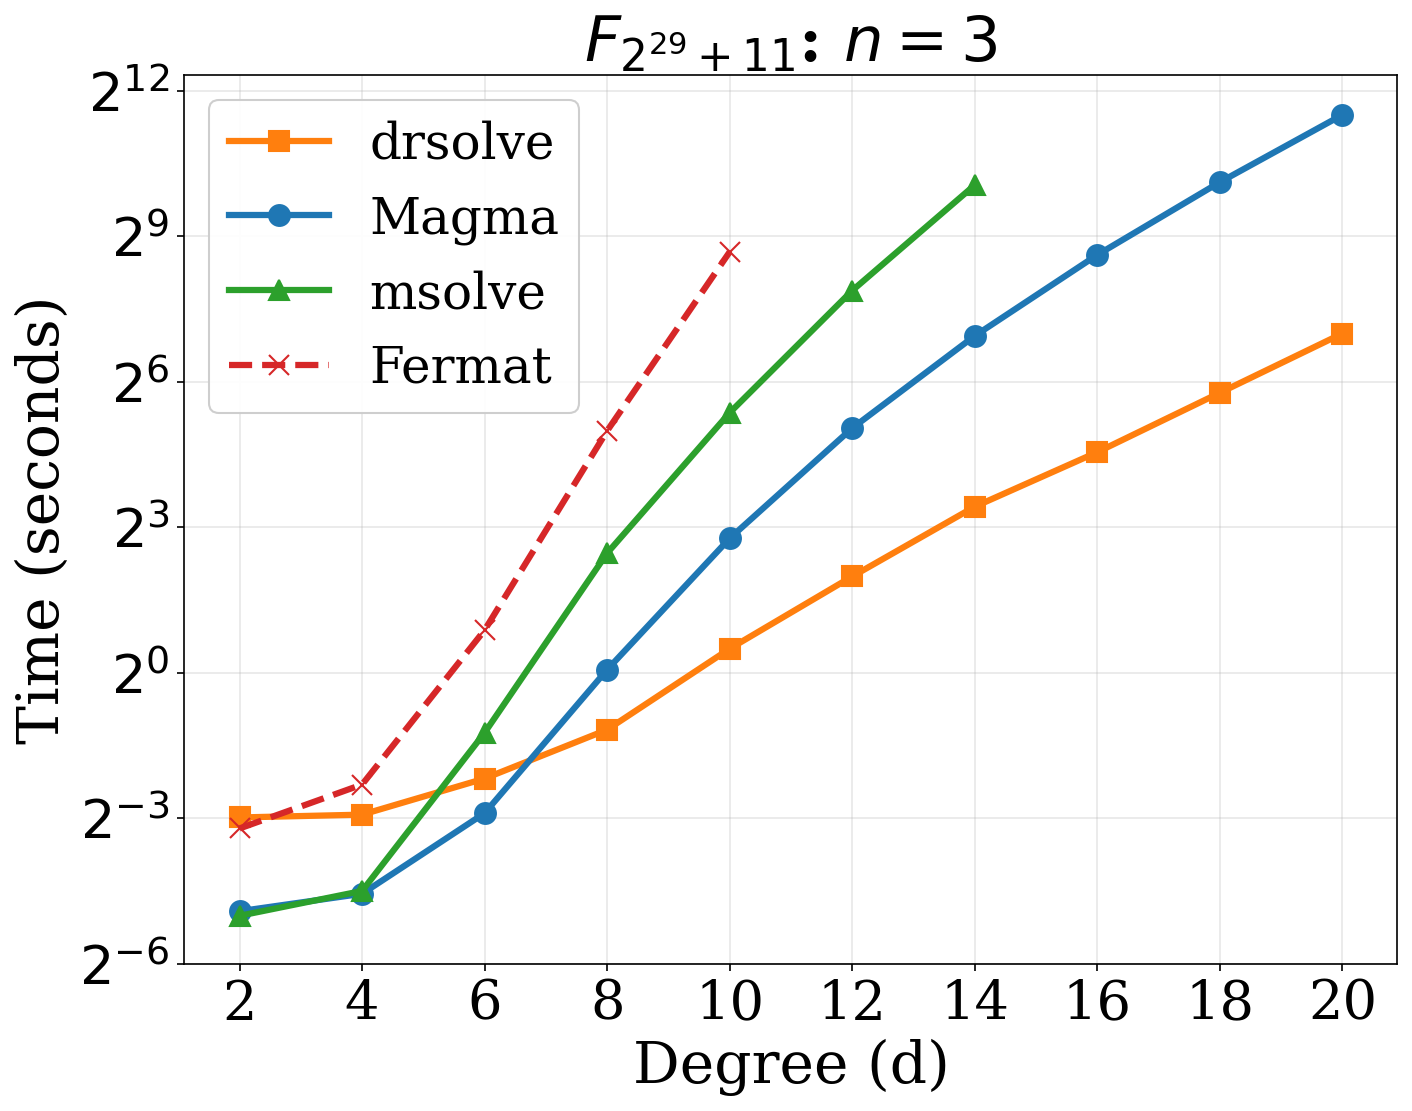
\includegraphics[width=\linewidth]{GF536870923_n3_comparison.png}
	\end{subfigure}\hfill
	\begin{subfigure}[t]{0.49\textwidth}
		\centering
		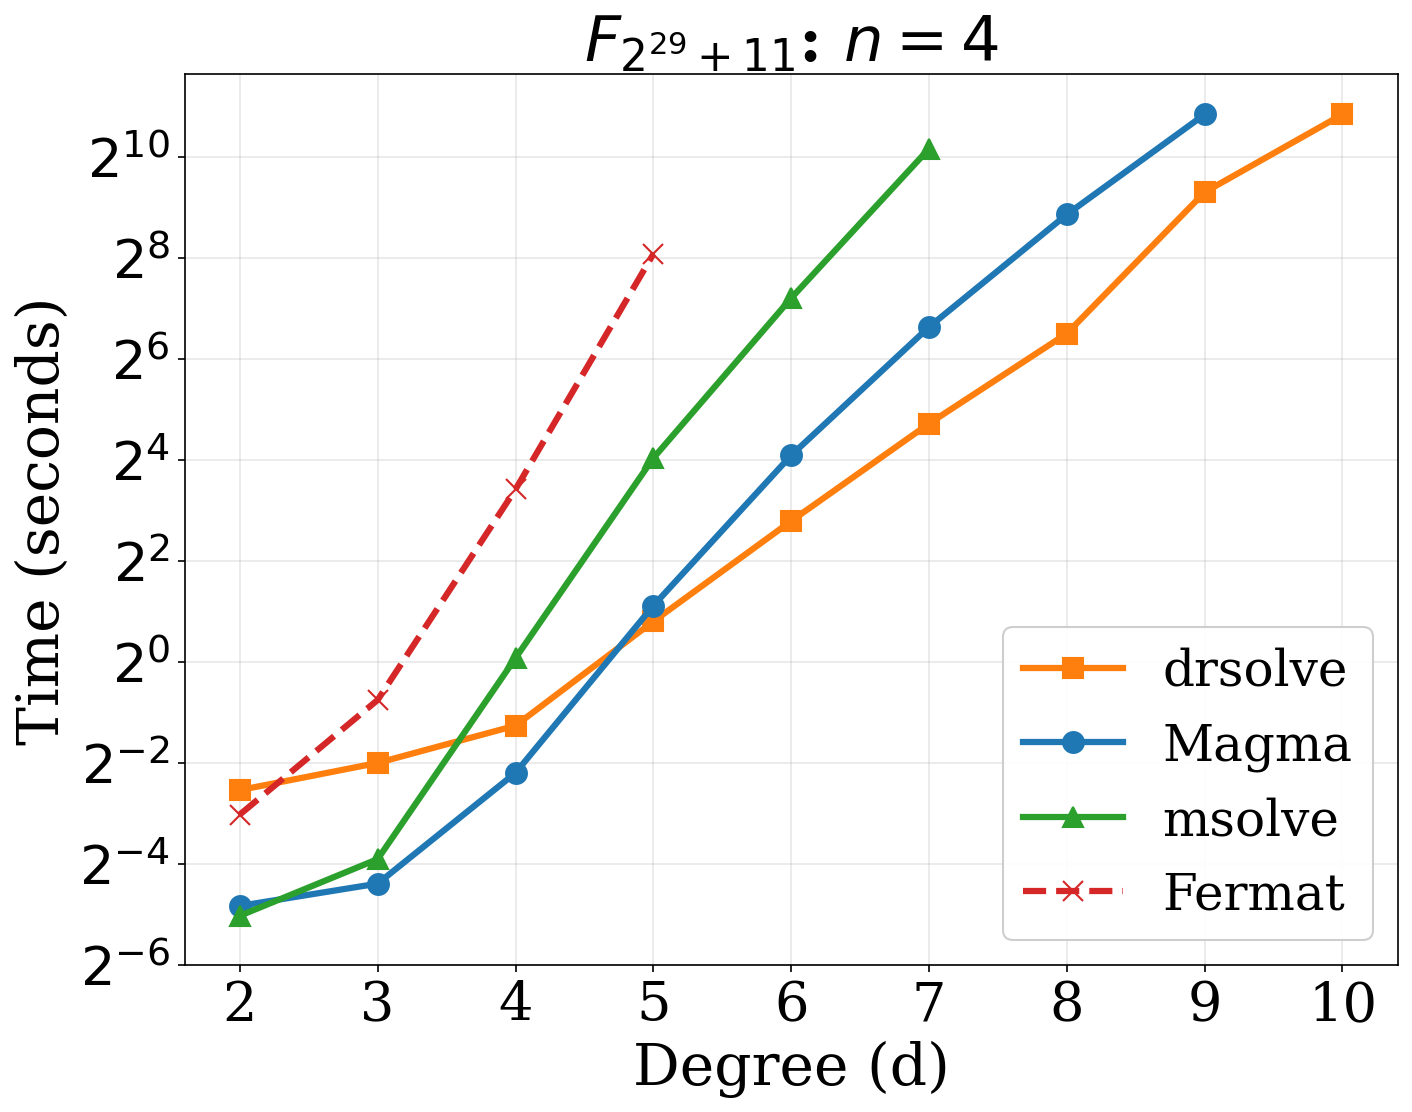
\includegraphics[width=\linewidth]{GF536870923_n4_comparison.png}
	\end{subfigure}\\[2pt]
	\begin{subfigure}[t]{0.49\textwidth}
		\centering
		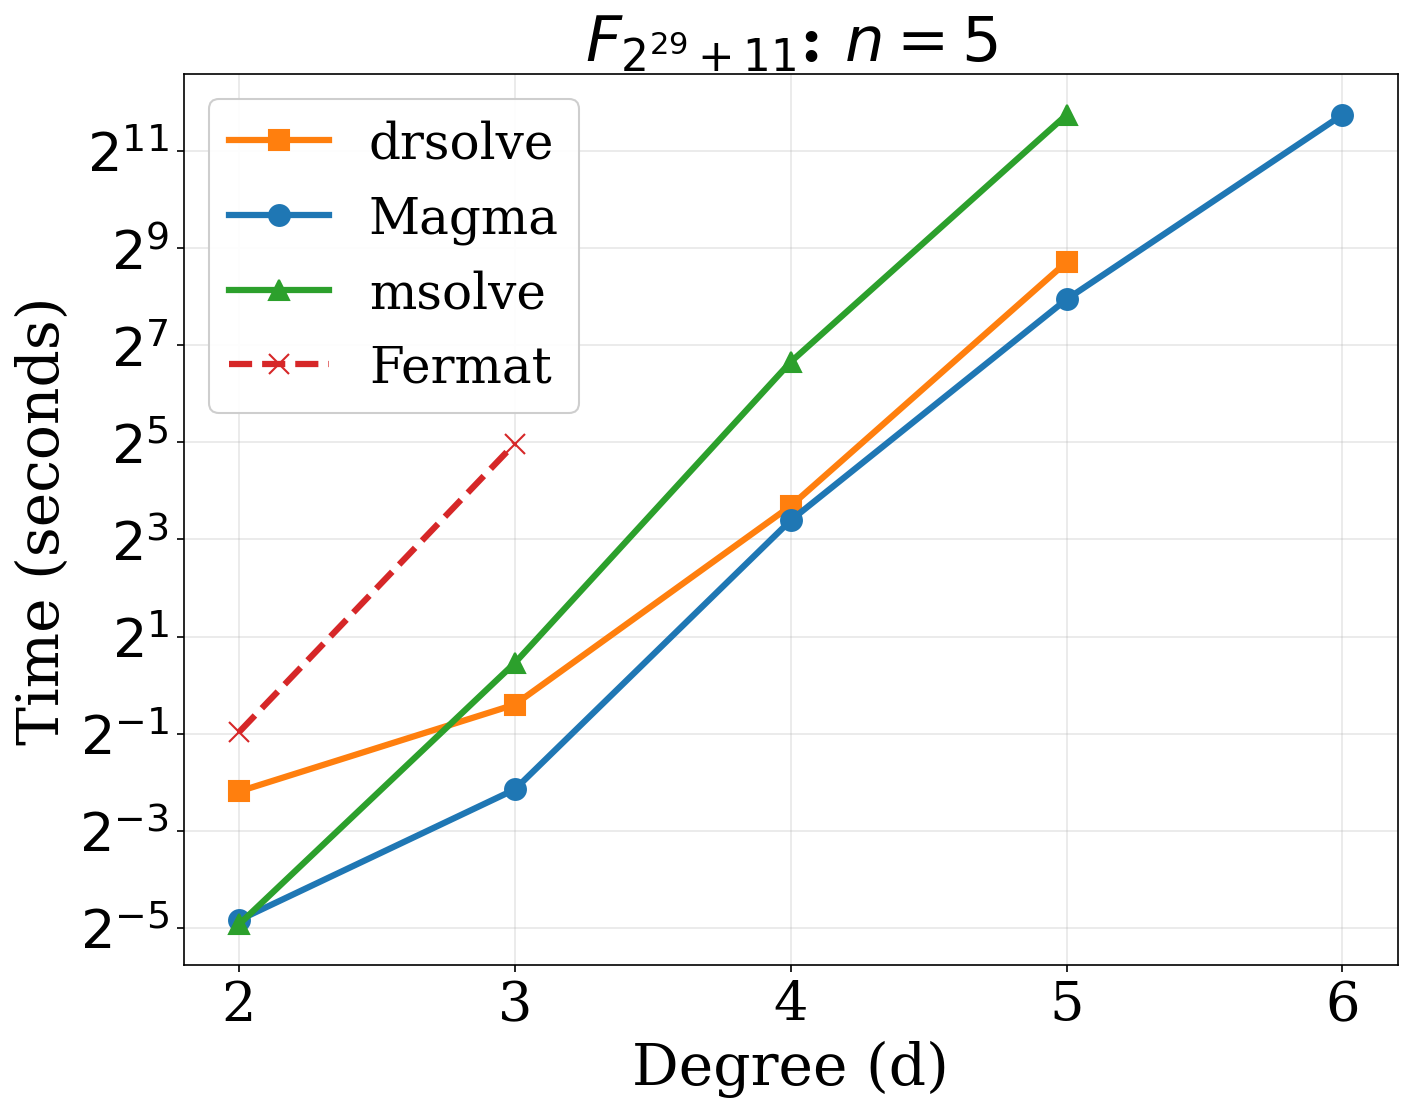
\includegraphics[width=\linewidth]{GF536870923_n5_comparison.png}
	\end{subfigure}\hfill
	\begin{subfigure}[t]{0.49\textwidth}
		\centering
		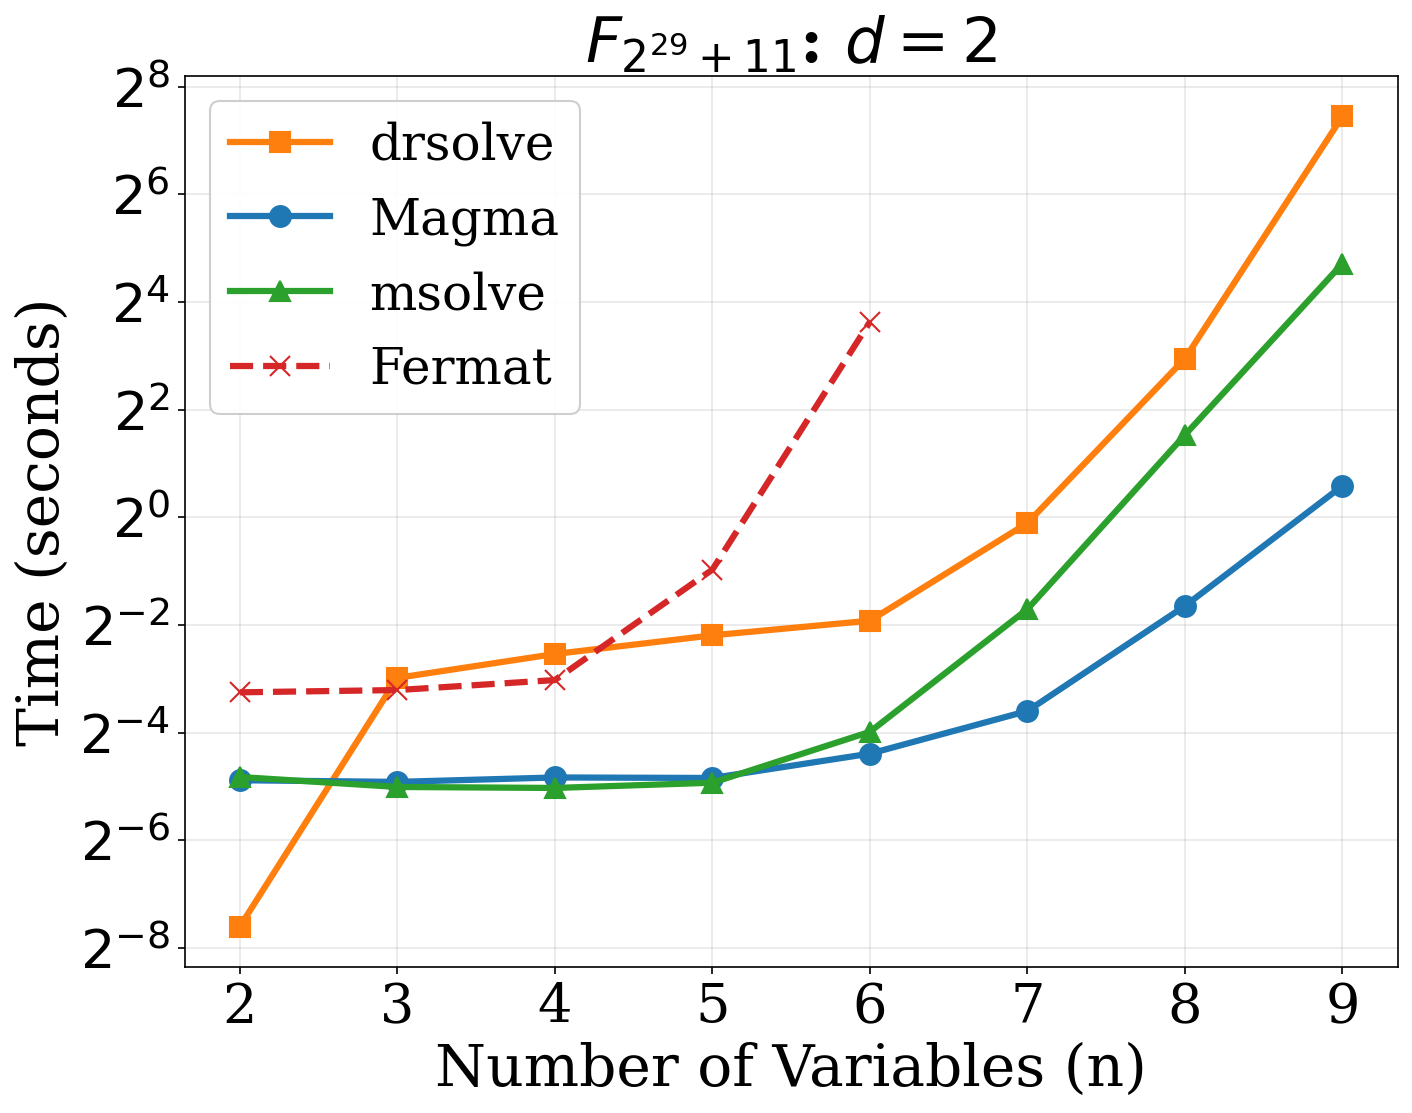
\includegraphics[width=\linewidth]{GF536870923_d2_vary_n.png}
	\end{subfigure}
	\caption{Performance comparison (time in seconds) of \drsolve, Magma, msolve, and Fermat on randomly generated dense polynomial systems over $\mathbb{F}_{2^{29}+11}$. The four panels show degree sweeps for $n=3,4,5$ and a variable-count sweep for $d=2$; here $n$ denotes the number of variables (equal to the number of equations). A curve stops where the corresponding solver exceeded the time or memory budget of the benchmark.}
	\label{fig:BenchmarkComparison}
\end{figure}




